\subsection{Sätze des Pythagoras}
\begin{Theorem}
  \begin{minipage}{0.5\textwidth}
    In einem rechtwingkligen Dreieck $\Delta ABC$ gilt:\\
    $$a^2+b^2=c^2$$
  \end{minipage}
  \begin{minipage}{0.5\textwidth}
    \definecolor{qqwuqq}{rgb}{0,0.39215686274509803,0}
    \definecolor{ududff}{rgb}{0.30196078431372547,0.30196078431372547,1}
    \begin{tikzpicture}[line cap=round,line join=round,>=triangle 45,x=1cm,y=1cm,scale=0.4]
    \clip(-13,-3) rectangle (0,4);
    \draw[line width=0.5pt,color=qqwuqq,fill=qqwuqq,fill opacity=0.10000000149011612] (-6.851258827998152,2.8478198196798843) -- (-6.633398787368505,2.627871663644841) -- (-6.413450631333462,2.8457317042744883) -- (-6.631310671963109,3.0656798603095314) -- cycle;
    \draw [line width=0.4pt] (-11.704106007375259,-1.9589560257157905)-- (-6.631310671963109,3.0656798603095314);
    \draw [line width=0.4pt] (-6.631310671963109,3.0656798603095314)-- (-1.6066747859377828,-2.007115475102615);
    \draw [line width=0.4pt] (-11.704106007375259,-1.9589560257157905)-- (-1.6066747859377828,-2.007115475102615);
    \begin{scriptsize}
    \draw [fill=ududff] (-11.704106007375259,-1.9589560257157905) circle (2.5pt);
    \draw[color=ududff] (-12,-1.646543156800932) node {$A$};
    \draw [fill=ududff] (-1.6066747859377828,-2.007115475102615) circle (2.5pt);
    \draw[color=ududff] (-1,-1.6903244744253179) node {$B$};
    \draw [fill=ududff] (-6.631310671963109,3.0656798603095314) circle (2.5pt);
    \draw[color=ududff] (-6.509790378375092,3.4) node {$C$};
    \draw[color=black] (-8.611293624345604,0.5425227244183474) node {$b$};
    \draw[color=black] (-4.831506536106975,0.5425227244183474) node {$a$};
    \draw[color=black] (-6.611946786165325,-1.7) node {$c$};
    \end{scriptsize}
    \end{tikzpicture}
  \end{minipage}
\end{Theorem}
\begin{Beweis}
  Man modelliere die 3 Seiten durch Vektoren, $\vv{a}$, $\vv{b}$ und $\vv{c}$.\\
  Es gilt: $$\vv{a} \cdot \vv{b} &= 0 $$
  $$ a_1 b_1+a_2 b_2 &= 0 $$
  Außerdem:
  \begin{center}
    \begin{align*}
      |\vv{a} + \vv{b}| &= \sqrt{(b_1-a_1)^2+(b_2-a_2)^2}\\
      &= \sqrt{{b_1}^2-2b_1 a_2+{a_1}^2 + {b_2}^2-2b_2 a_2+{a_2}^2}\\
      &= \sqrt{{b_1}^2 + {b_2}^2 + {a_1}^2 + {a_2}^2 -2(b_1 a_2 + b_2 a_2)}\\
      &= \sqrt{{b_1}^2 + {b_2}^2 + {a_1}^2 + {a_2}^2}\\
      &= |\vv{c}| \text{, denn $\vv{a} + \vv{b} = \vv{c}$}\\
      \Leftrightarrow |\vv{c}|^2 &= {b_1}^2 + {b_2}^2 + {a_1}^2 + {a_2}^2\\
      \Leftrightarrow |\vv{c}|^2 &= |\vv{a}|^2 + |\vv{b}|^2\\
      \Leftrightarrow c^2 &= a^2 + b^2\\
    \end{align*}
  \end{center}
\end{Beweis}
\begin{Bemerkung}
  Dieser Beweis ist weitaus intuitiver und einfacher, wenn er in der klasischen Geometrie vollführt wird, aber unser Ziel ist es die vorliegenden Sätze über Vektoren, und damit analytisch zu beweisen.
\end{Bemerkung}
\begin{Theorem}[- Umkehrung]
  \begin{minipage}{0.5\textwidth}
    Falls für ein Dreieck $\Delta ABC$ gilt:\\
    $$a^2+b^2=c^2$$
    Dann ist dieses Dreieck in $C$ rechtwinklig.
  \end{minipage}
  \begin{minipage}{0.5\textwidth}
    \definecolor{qqwuqq}{rgb}{0,0.39215686274509803,0}
    \definecolor{ududff}{rgb}{0.30196078431372547,0.30196078431372547,1}
    \begin{tikzpicture}[line cap=round,line join=round,>=triangle 45,x=1cm,y=1cm,scale=0.4]
    \clip(-13,-3) rectangle (0,4);
    \draw[line width=0.5pt,color=qqwuqq,fill=qqwuqq,fill opacity=0.10000000149011612] (-6.851258827998152,2.8478198196798843) -- (-6.633398787368505,2.627871663644841) -- (-6.413450631333462,2.8457317042744883) -- (-6.631310671963109,3.0656798603095314) -- cycle;
    \draw [line width=0.4pt] (-11.704106007375259,-1.9589560257157905)-- (-6.631310671963109,3.0656798603095314);
    \draw [line width=0.4pt] (-6.631310671963109,3.0656798603095314)-- (-1.6066747859377828,-2.007115475102615);
    \draw [line width=0.4pt] (-11.704106007375259,-1.9589560257157905)-- (-1.6066747859377828,-2.007115475102615);
    \begin{scriptsize}
    \draw [fill=ududff] (-11.704106007375259,-1.9589560257157905) circle (2.5pt);
    \draw[color=ududff] (-12,-1.646543156800932) node {$A$};
    \draw [fill=ududff] (-1.6066747859377828,-2.007115475102615) circle (2.5pt);
    \draw[color=ududff] (-1,-1.6903244744253179) node {$B$};
    \draw [fill=ududff] (-6.631310671963109,3.0656798603095314) circle (2.5pt);
    \draw[color=ududff] (-6.509790378375092,3.4) node {$C$};
    \draw[color=black] (-8.611293624345604,0.5425227244183474) node {$b$};
    \draw[color=black] (-4.831506536106975,0.5425227244183474) node {$a$};
    \draw[color=black] (-6.611946786165325,-1.7) node {$c$};
    \end{scriptsize}
    \end{tikzpicture}
  \end{minipage}
\end{Theorem}
\begin{Beweis}
  test
\end{Beweis}

\subsection{Euklids Sätze}
\begin{Theorem}[- Kathetensatz]
  \begin{minipage}{0.5\textwidth}
  In einem in $C$ rechtwinkligen Dreieck $\Delta ABC$ mit $h$ der Höhe zu $C$ gilt:\\
    \begin{itemize}
      \item $a^2 = p \cdot c$
      \item $b^2 = q \cdot c$
    \end{itemize}
  \end{minipage}
  \begin{minipage}{0.5\textwidth}
    \definecolor{qqwuqq}{rgb}{0,0.39215686274509803,0}
    \definecolor{ududff}{rgb}{0.30196078431372547,0.30196078431372547,1}
    \begin{tikzpicture}[line cap=round,line join=round,>=triangle 45,x=1cm,y=1cm,scale=.6]
    \clip(-8.311937785825172,-3) rectangle (8.290449729798194,2);
    \draw [shift={(-3.5656013566444793,1.3718053107067734)},line width=0.5pt,color=qqwuqq,fill=qqwuqq,fill opacity=0.16] (0,0) -- (-120.15054216593154:0.48766804060251406) arc (-120.15054216593154:-30.15055075070568:0.48766804060251406) -- cycle;
    \draw [line width=0.4pt] (-5.890547931937073,-2.630796139481519)-- (-3.5656013566444793,1.3718053107067734);
    \draw [line width=0.4pt] (3.459368369267905,-2.708712108658227)-- (-3.5656013566444793,1.3718053107067734);
    \draw [line width=0.4pt] (-5.890547931937073,-2.630796139481519)-- (3.459368369267905,-2.708712108658227);
    \draw [line width=0.4pt] (-3.5656013566444793,1.3718053107067734)-- (-3.5991154959818794,-2.6498914097811452);
    \draw [line width=0.4pt] (-5.890547931937073,-2.630796139481519)-- (-3.5991154959818794,-2.6498914097811452);
    \draw [line width=0.4pt] (3.459368369267905,-2.708712108658227)-- (-3.5991154959818794,-2.6498914097811452);
    \begin{scriptsize}
    \draw [fill=ududff] (-5.890547931937073,-2.630796139481519) circle (2.5pt);
    \draw[color=ududff] (-6.1,-2.3936022538574075) node {$A$};
    \draw [fill=ududff] (3.459368369267905,-2.708712108658227) circle (2.5pt);
    \draw[color=ududff] (3.543814134600391,-2.43) node {$B$};
    \draw [fill=ududff] (-3.5656013566444793,1.3718053107067734) circle (2.5pt);
    \draw[color=ududff] (-3.4786056500758114,1.8) node {$C$};
    \draw[color=black] (-4.9,-0.583811969844107) node {$b$};
    \draw[color=black] (0.07595251253806888,-0.38874475360315236) node {$a$};
    \draw[color=black] (-1.8638825823030425,-2.9) node {$c$};
    \draw[color=black] (-3.75,-0.5079524968615136) node {$h$};
    \draw[color=black] (-4.605660677246067,-2.328579848443756) node {$q$};
    \draw[color=black] (-0.03241816315137868,-2.3719281187195236) node {$p$};
    \end{scriptsize}
    \end{tikzpicture}
  \end{minipage}
\end{Theorem}
\begin{Beweis}
  test
\end{Beweis}
\begin{Theorem}[- Höhensatz]
  \begin{minipage}{0.5\textwidth}
    In einem in $C$ rechtwinkligen Dreieck $\Delta ABC$ mit $h$ der Höhe zu $C$ gilt:
    $$h^2=p\cdot q$$
  \end{minipage}
  \begin{minipage}{0.5\textwidth}
    \definecolor{qqwuqq}{rgb}{0,0.39215686274509803,0}
    \definecolor{ududff}{rgb}{0.30196078431372547,0.30196078431372547,1}
    \begin{tikzpicture}[line cap=round,line join=round,>=triangle 45,x=1cm,y=1cm,scale=.6]
    \clip(-8.311937785825172,-3) rectangle (8.290449729798194,2);
    \draw [shift={(-3.5656013566444793,1.3718053107067734)},line width=0.5pt,color=qqwuqq,fill=qqwuqq,fill opacity=0.16] (0,0) -- (-120.15054216593154:0.48766804060251406) arc (-120.15054216593154:-30.15055075070568:0.48766804060251406) -- cycle;
    \draw [line width=0.4pt] (-5.890547931937073,-2.630796139481519)-- (-3.5656013566444793,1.3718053107067734);
    \draw [line width=0.4pt] (3.459368369267905,-2.708712108658227)-- (-3.5656013566444793,1.3718053107067734);
    \draw [line width=0.4pt] (-5.890547931937073,-2.630796139481519)-- (3.459368369267905,-2.708712108658227);
    \draw [line width=0.4pt] (-3.5656013566444793,1.3718053107067734)-- (-3.5991154959818794,-2.6498914097811452);
    \draw [line width=0.4pt] (-5.890547931937073,-2.630796139481519)-- (-3.5991154959818794,-2.6498914097811452);
    \draw [line width=0.4pt] (3.459368369267905,-2.708712108658227)-- (-3.5991154959818794,-2.6498914097811452);
    \begin{scriptsize}
    \draw [fill=ududff] (-5.890547931937073,-2.630796139481519) circle (2.5pt);
    \draw[color=ududff] (-6.1,-2.3936022538574075) node {$A$};
    \draw [fill=ududff] (3.459368369267905,-2.708712108658227) circle (2.5pt);
    \draw[color=ududff] (3.543814134600391,-2.43) node {$B$};
    \draw [fill=ududff] (-3.5656013566444793,1.3718053107067734) circle (2.5pt);
    \draw[color=ududff] (-3.4786056500758114,1.8) node {$C$};
    \draw[color=black] (-4.9,-0.583811969844107) node {$b$};
    \draw[color=black] (0.07595251253806888,-0.38874475360315236) node {$a$};
    \draw[color=black] (-1.8638825823030425,-2.9) node {$c$};
    \draw[color=black] (-3.75,-0.5079524968615136) node {$h$};
    \draw[color=black] (-4.605660677246067,-2.328579848443756) node {$q$};
    \draw[color=black] (-0.03241816315137868,-2.3719281187195236) node {$p$};
    \end{scriptsize}
    \end{tikzpicture}
  \end{minipage}
\end{Theorem}
\begin{Beweis}
  test
\end{Beweis}

\subsection{Strahlensätze}
\begin{Theorem}
  \begin{minipage}{0.5\textwidth}
    Sei ein Dreieck $\Delta ABC$ mit M einem Punkt der Geraden $(AB)$ und N einem Punkt der Geraden $(AC)$. Wenn $(BC)//(MN)$, dann gilt:\\
    $$\dfrac{AM}{AB}=\dfrac{AN}{AC}=\dfrac{MN}{BC}$$
  \end{minipage}
  \begin{minipage}{0.5\textwidth}

  \end{minipage}
\end{Theorem}
\begin{Beweis}
  test
\end{Beweis}
Die Umkehrung dieses Satzes:
\begin{Theorem}
  \begin{minipage}{0.5\textwidth}
  Sei ein Dreieck $\Delta ABC$ mit M einem Punkt der Geraden $(AB)$ und N einem Punkt der Geraden $(AC)$. Wenn gilt:\\
  $$\dfrac{AB}{AC}=\dfrac{AM}{AN}$$
    Dann ist $(BC)//(MN)$.
  \end{minipage}
  \begin{minipage}{0.5\textwidth}
    draw
  \end{minipage}
\end{Theorem}
\begin{Beweis}
  test
\end{Beweis}

\subsection{Der Satz des Apollinius}
\begin{Definition}
  \begin{minipage}[t]{0.5\textwidth}
    Gegeben sind: Eine Strecke $[AB]$ und eine positive Zahl $\lambda \in \R^{+} \backslash \{1\}$. Dann ist die Punktmenge $$M_{A}=\{X| \dfrac{\overline{AX}} {\overline{XB}}=\lambda \}$$ ein Kreis, den man \textbf{Kreis des Apollinius} nennt.
  \end{minipage}
  \begin{minipage}[t]{0.5\textwidth}
    \center{Anschaulich:}\\
    \definecolor{xdxdff}{rgb}{0.49019607843137253,0.49019607843137253,1}
    \begin{tikzpicture}[line cap=round,line join=round,>=triangle 45,x=1cm,y=1cm,scale=0.4]
      \clip(-15.430804837667225,-8) rectangle (6.387208662312055,4);
      \draw [line width=0.6pt] (-3.467268565272,-2.1740714480434544) circle (4.233988972549521cm);
      \draw [line width=0.6pt] (-6.695919714230329,0.5649930597768731)-- (-5.612633124394338,-2.1755042586210407);
      \draw [line width=0.6pt] (-6.695919714230329,0.5649930597768731)-- (-13.088243523450211,-2.180496945578665);
      \draw [line width=0.6pt] (-13.088243523450211,-2.180496945578665)-- (0.766719463010253,-2.171243722188424);
      \begin{scriptsize}
      \draw [fill=xdxdff] (-6.695919714230329,0.5649930597768731) circle (2pt);
      \draw[color=xdxdff] (-6.4308742689257725,1.3147960193295674) node {$X$};
      \draw [fill=xdxdff] (0.766719463010253,-2.171243722188424) circle (2pt);
      \draw[color=xdxdff] (1.137249163879541,-1.3442743759804054) node {$T_a$};
      \draw [fill=xdxdff] (-5.612633124394338,-2.1755042586210407) circle (2pt);
      \draw[color=xdxdff] (-5.339973593926808,-1.4465463142615582) node {$B$};
      \draw [fill=xdxdff] (-13.088243523450211,-2.180496945578665) circle (2pt);
      \draw[color=xdxdff] (-12.805825088450968,-1.4465463142615582) node {$A$};
      \draw [fill=xdxdff] (-7.701256593554253,-2.1768991738984846) circle (2pt);
      \draw[color=xdxdff] (-7,-1.4124556681678406) node {$T_i$};
      \end{scriptsize}
    \end{tikzpicture}
  \end{minipage}
  Der Satz besagt also, dass alle Punkte $X$ deren Abst"ande zu $A$ ($\overline{AX}$) und zu $B$ ($\overline{XB}$) im Verh"altnis $\lambda$ stehen, auf einem Kreis liegen.\\
\end{Definition}
\begin{Beweis}
  Anfangen kann man den den Beweis damit, dass man zwei Punkte sucht, die die Bedingung erf"ullen \textbf{und} auf der Geraden $AB$ liegen. Logisch ist, dass einer dieser Punkte zwischen $A$ und $B$ sein wird, dieser wird \textbf{innerer Teilungspunkt} $T_{i}$ genannt. Der andere Punkt liegt au"serhalb der Strecke $[AB]$ und wird \textbf{"au"serer Teilungspunkt} $T_{a}$ genannt. \\
  Im letzten Schritt des Beweises wird man anhand des Skalarprodukts zeigen, dass f"ur alle Punkte $X$, die ebenfalls die Verh"altnisgleichung erf"ullen, die Vektoren $\vv{T_{i}X}$ und $\vv{T_{a}X}$ orthogonal zueinander sind. Somit liegen diese Punkte auf dem Thaleskreis (frz.: Theoreme du triangle rectangle) "uber $T_{i}$ und $T_{a}$, der dann \textbf{Apolliniuskreis} genannt wird.\\
  \begin{enumerate}


  \item {Um uns die Arbeit so einfach wie m"oglich zu machen, platzieren wir unseren ersten Punkt $A$ auf den Ursprung eines Koordinatensystems und die Strecke $[AB]$ entlang der $x$-Achse . Der Punkt $B$ hat den Abstand $\overline{AB}$ zu $A$, den man $b$ abk"urzt. Gleicherma"sen verf"ahrt man mit den L"angen $\overline{AT_{i}}=t_{i}$ und $\overline{AT_{a}}= t_{a}$, und man f"uhrt den Punkt $X(x|y)$ ein.\\
  Hier nochmal ein "Uberblick:\\
  \\
  \vartriangleright $A(0|0)$ \qquad \vartriangleright $B(b|0)$ \qquad \vartriangleright $T_{i}(t_{i}|0)$ \qquad \vartriangleright $T_{a}(t_{a}|0)$ \qquad \vartriangleright $X(x|y)$\\
  \\}

  \item {Nun gilt:
  \begin{center}
  $\dfrac{\overline{AT_{i}}}{\overline{T_{i}B}} = \lambda$ \qquad und \qquad $\dfrac{\overline{AT_{a}}}{\overline{T_{a}B}} = \lambda$ \\
  \end{center}
  Das benutzt man, um die Koordinaten $t_{i}$ und $t_{a}$ in Abh"angigkeit von $b$ und $\lambda$ auszudr"ucken, denn diese Punkte sind ja durch das Verh"altnis $\lambda$ in der Ebene festgelegt.\\

  \begin{minipage}[t]{0.5\textwidth}
  \begin{array}{rccl}
  &$\dfrac{\overline{AT_{i}}}{\overline{T_{i}B}}$ & $=$ & $\lambda$\\
  $\Leftrightarrow & \dfrac{t_{i}}{b-t_{i}} $& $= $& $\lambda$\\
  $\Leftrightarrow & $t_{i}$&$=$&$\lambda \cdot b - \lambda \cdot t_{i}$\\
  $\Leftrightarrow & \lambda \cdot t_{i} + t_{i}$ &$=$& \lambda \cdot b$\\
  $\Leftrightarrow & (\lambda + 1)\cdot t_{i}$&$=$& $\lambda \cdot b$\\
  $\Leftrightarrow & t_{i} $&$=$& $ \dfrac {\lambda}{\lambda +1}\cdot b$
  \end{array}
  \end{minipage}
  \begin{minipage}[t]{0.5\textwidth}
  \begin{array}{rccl}
  &$\dfrac{\overline{AT_{a}}}{\overline{T_{a}B}} $&$ = $&$ \lambda$\\
  $\Leftrightarrow $&$ \dfrac{t_{a}}{t_{a}-b} $&$ = $& $\lambda$\\
  $\Leftrightarrow & $t_{a}$&$=$&$\lambda \cdot t_{a} - \lambda \cdot b$\\
  $\Leftrightarrow & \lambda \cdot t_{a} - t_{a} $&$=$&$\lambda \cdot b$\\
  $\Leftrightarrow & (\lambda -1 \cdot )t_{a} $&$=$&$\lambda \cdot b$\\
  $\Leftrightarrow & t_{a} $&$=$&$ \dfrac{\lambda}{\lambda -1}\cdot b$\\
  \end{array}
  \end{minipage}}
  \\
  \item{ Jetzt wo wir $T_{i}$ und $T_{a}$ in Abh"angigkeit von $b$ und $\lambda$ bestimmt haben, kann man die Vorraussetzung auch noch auf den Punkt $X$ anwenden.\\
  \\
  \begin{array}{rcccl}
  &$\dfrac{\overline{AX}}{\overline{XB}}$ & $=$ & $\lambda$ \\
  $\Leftrightarrow & $(\dfrac{\overline{AX}}{\overline{XB}})^2$ & $=$ & \lambda^2$\\
  $\Leftrightarrow & $\dfrac{(\overline{AX})^2}{(\overline{XB})^2}$ & $=$ & \lambda^2$\\
  $\Leftrightarrow & $\dfrac{x^2+y^2}{(x-b)^2+y^2} $ & $=$ & $\lambda^2$\\
  $\Leftrightarrow & $x^2+y^2$ & $=$ & $\lambda^2 \cdtot [(x-b)^2+y^2]$\\
  $\Leftrightarrow & $0$ & $=$ & $\lambda^2 \cdot (x-b)^2 +\lambda^2 y^2 -x^2 -y^2$\\
  $\Leftrightarrow & $0$ & $=$ & $x^2\cdot \lambda^2 - 2bx\cdot \lambda^2 +b^2\cdot \lambda^2 +y^2\cdot \lambda^2 -x^2-y^2 $ &\textcolor{red}{(1)}\\
  \\
  \end{array}
  }



  \item{
  Bevor man zum Ende kommt, kann man noch die Ergebnisse aus 2) benutzen, um $t_{i}$ und $t_{a}$ miteinander zu verrechnen, denn diesen Zusammenhang braucht man gleich.\\
  \begin{center}
  \begin{array} {rccccccl}
  $t_{i} + t_{a} $ & $=$ & $\dfrac {\lambda}{\lambda +1}\cdot b + $\dfrac {\lambda}{\lambda -1}\cdot b  $ &$=$& $(\dfrac{\lambda}{\lambda+1} + \dfrac{\lambda}{\lambda-1})\cdot b$ & $=$ & $\dfrac{\lambda^2}{\lambda^2 -1}\cdot 2b$ \qquad \textcolor{red}{(2)}\\
  \end{array}
  \\
  \begin{array} {rcccccl}
  $t_{i} \cdot t_{a} $ & $=$ & $\dfrac {\lambda}{\lambda +1}\cdot b \cdot $\dfrac {\lambda}{\lambda +1}\cdot b $ & $=$ & $\dfrac{\lambda^2}{\lambda^2 -1}\cdot b^2$ \qquad \textcolor{red}{(3)}\\ \\
  \end{array}
  \end{center}
  }

  \item{
  Nun kommt der finale Schritt. Man bildet die Vektoren $\vv{T_{i}X} = \left(\begin{array}{c} x-t_{i} \\ y \end{array}\right)$ und $\vv{T_{a}X} = \left(\begin{array}{c} x-t_{a} \\ y \end{array}\right)$ und berechnet deren Skalarprodukt. $\ast$ TROMMELWIRBEL$\ast$ \\
  \\
  \begin{center}
  \begin{array}{rccl}
  $\vv{T_{i}X} \cdot \vv{T_{a}X}$ &$=$& $(x-t_{i})\cdot (x-t_{a}) +y^2$\\
  & $=$ & $x^2 -(t_{i} +t_{a})x + t_{i}\cdot t_{a} + y^2$ & $Benutze (2) und (3) \\
  & $=$ & $x^2 - \dfrac{\lambda^2}{\lambda^2 - 1} \cdot 2bx + \dfrac{\lambda^2}{\lambda^2 - 1} \cdot b^2 +y^2$\\
  & $=$ & $\dfrac{x^2 \cdot (\lambda^2 -1) - 2bx\cdot \lambda^2 + b^2\cdot \lambda^2 + y^2 \cdot (\lambda^2 -1)}{\lambda^2 -1}$\\
  & $=$ & $\dfrac{x^2 \cdot \lambda^2 - 2bx\cdot \lambda^2 b^2\cdot \lambda^2 +y^2\cdot \lambda^2 -x^2 -y^2} {\lambda^2 -1}$ &  $Benutze (1) \\
  & $=$ & $0$\\
  \\
  \end{array}
  \end{center}
  }

  Damit hat man bewiesen, dass f"ur alle Punkte $X$ die Vektoren $\vv{T_{i}X}$ und $\vv{T_{a}X}$ orthogonal zueinander sind, weshalb sie auf dem Thaleskreis "uber $T_{i}$ und $T_{a}$ liegen m"ussen.\\ \\
  \end{enumerate}
\end{Beweis}


Die Figur und die Zusammenh"ange, die man durch den Satz des Apollinius erhalten hat, kann man benutzen, um ein wenig mit Winkeln zu spielen: \\
\\
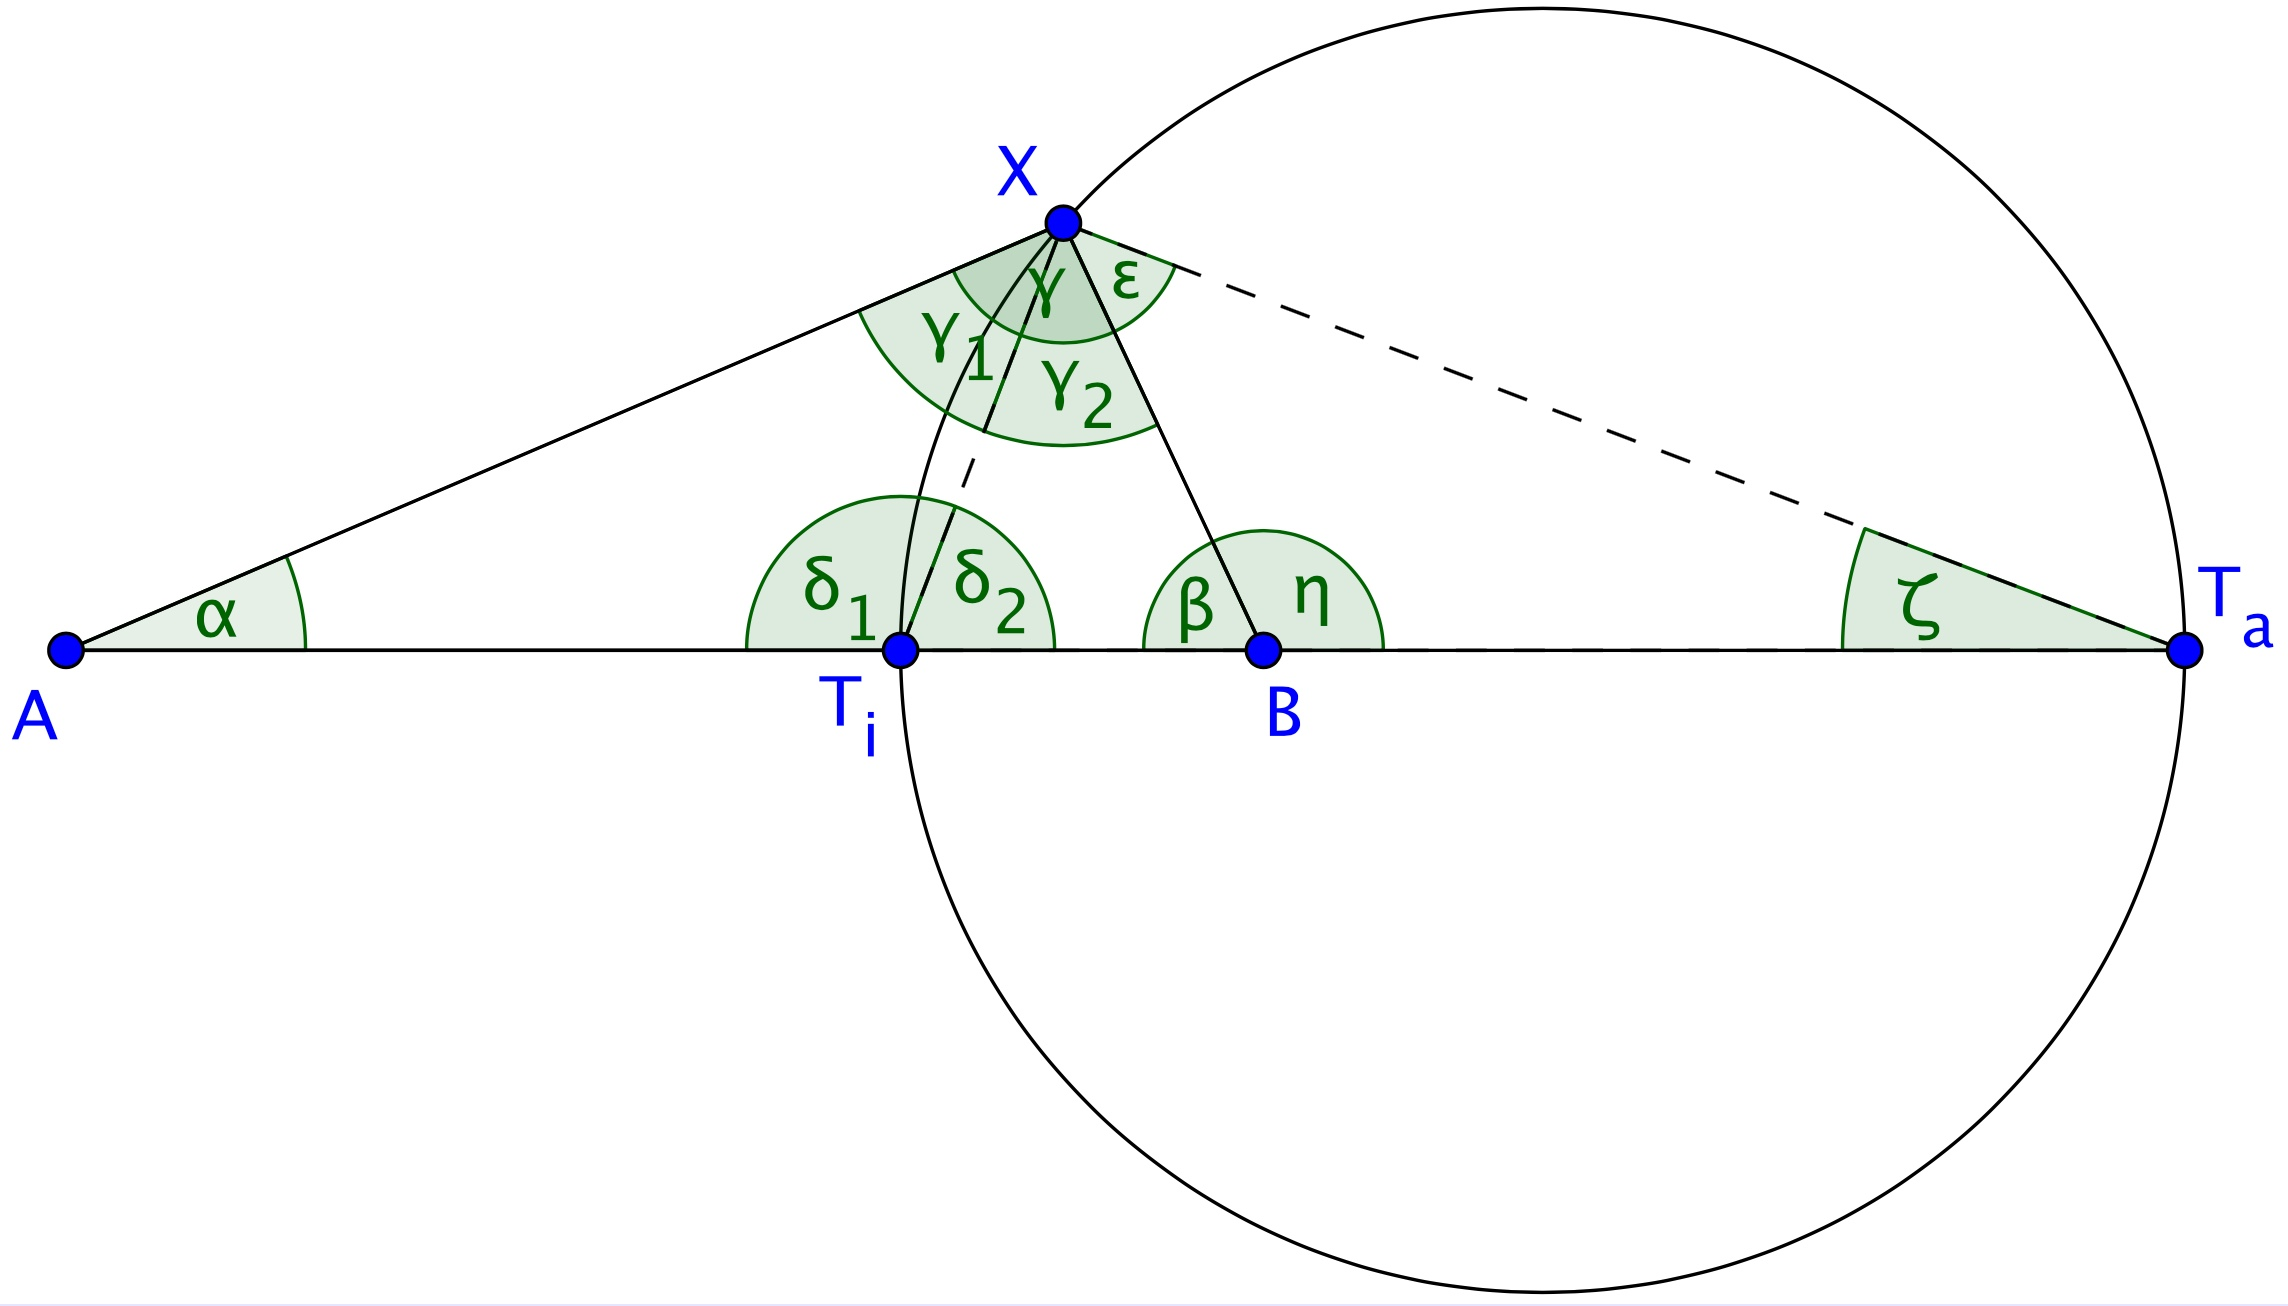
\includegraphics[width=5in]{kap5/Apollinius_Winkel}\\
\\
\begin{mdframed}
Auf dieser Skizze sind 10 Winkel gekennzeichnet, zu welchen sich eine ganze Reihe von Beziehungen aufstellen l"asst:\\
\\
\begin{array}{rcccl}
$\vartriangleright \alpha + \beta + \gamma = 180 $ & $\vartriangleright \beta + \gamma_{2} + \delta_{2} = \ang{180} $ & $\vartriangleright \delta_{1} + \delta_{2} = \ang{180} $ & $\vartriangleright \alpha + \gamma + \epsilon + \zeta = \ang{180} $ &$\vartriangleright \epsilon + \zeta + \eta = \ang{180}$\\
$\vartriangleright \aplha + \gamma_{1} + \delta_{1} = \ang{180} $ & $\vartriangleright \gamma_{1} + \gamma_{2} = \gamma $ & $\vartriangleright \gamma_{2} + \epsilon = \ang{90} $ & $\vartriangleright \beta + \eta = \ang{180} $ &$\vartriangleright \gamma_{2} + \delta_{2} + \epsilon + \zeta = \ang{180}$\\
\\
\end{array}
\\
Hiermit bekommt man ein zehndimensionales Gleichungssystem mit dem sich $\gamma_{1} = \gamma_{2}$ zeigen l"asst. Dies bedeutet dass die Gerade $T_{i}X$ auch noch die Winkelhalbierende des Winkels $\gamma = \angle AXB$ ist:
\\
\end{mdframed}
\begin{Definition}
  Eine Innenwinkelhalbierende eines Dreiecks teilt die gegen"uberliegende Seite im Verh"altnis der Anliegenden Seiten. \qquad $\gamma_{1}=\gamma_{2} \Rightarrow \overline{AT_{i}}:\overline{T_{i}B}=\overline{AX}:\overline{XB}$\\
  \tiny{Quelle: Skript 1ere SBC S.68-71, 06.03.18, Tobias Rave}
\end{Definition}
 \begin{center}
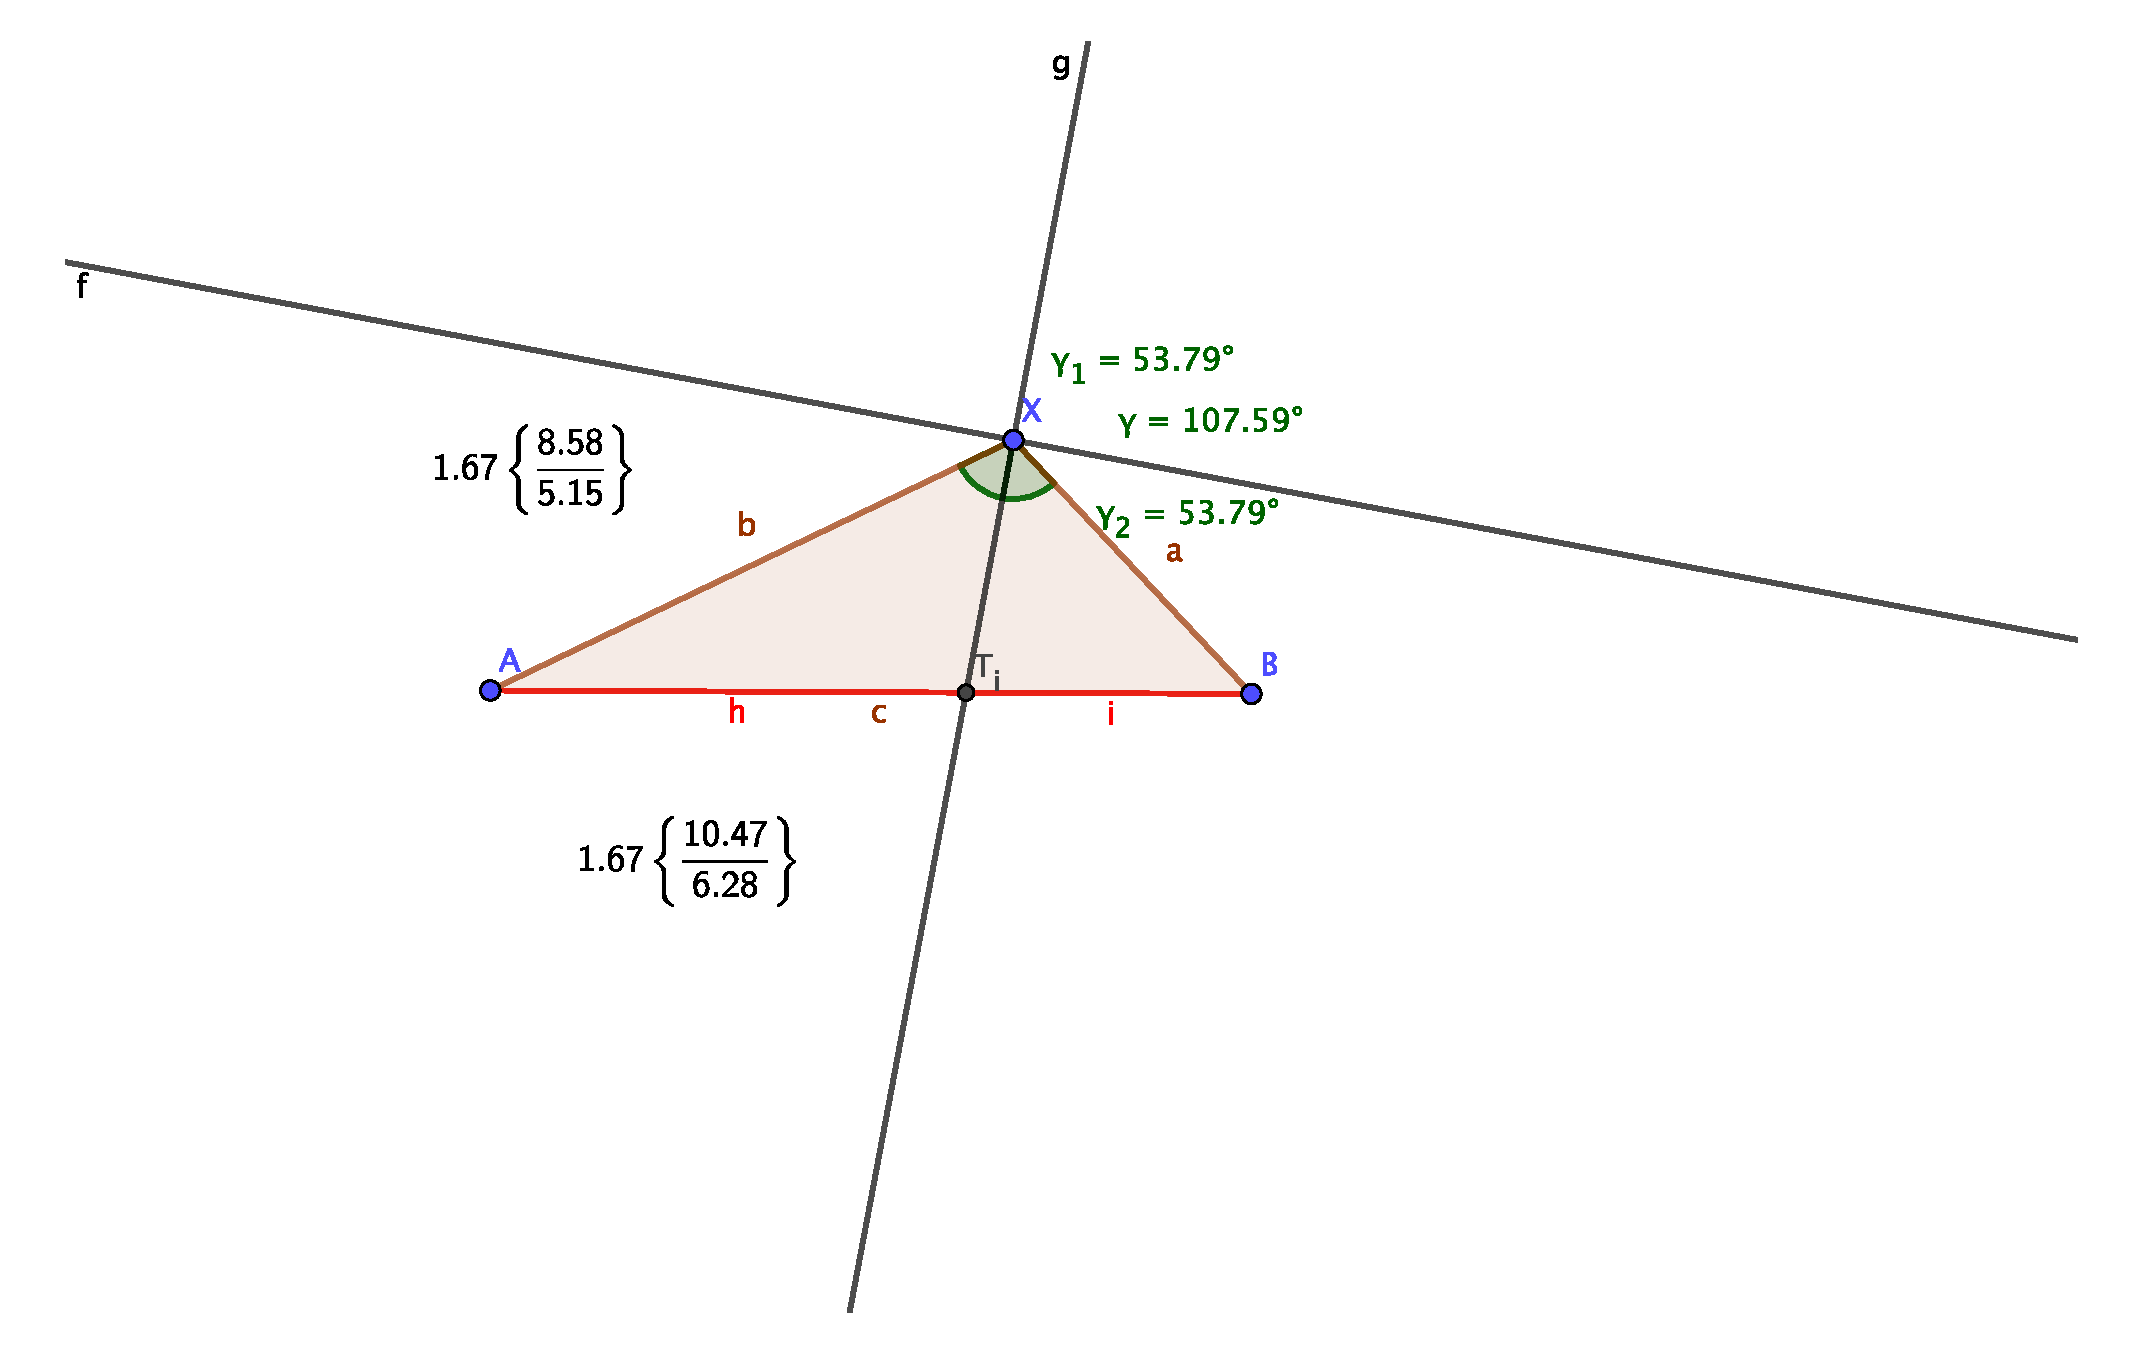
\includegraphics[width=4.7in]{kap5/Apollinus_Winkelhalbierende_Bild.pdf}
\end{center}
\end{small}
